\documentclass[aspectratio=169]{beamer}
\usepackage[utf8]{inputenc}
\usepackage[T1]{fontenc}
\usepackage[spanish,es-tabla]{babel}
\usepackage{graphicx,booktabs,array}
\usepackage{amsmath}
\usepackage{xcolor}
\usepackage{hyperref}

\graphicspath{{images/}}
\hypersetup{hidelinks}

\definecolor{ink}{HTML}{111111}
\definecolor{gray}{HTML}{666666}
\definecolor{rulegray}{HTML}{CCCCCC}
\definecolor{pale}{HTML}{F2F2F2}
\definecolor{blue}{HTML}{2F66A7}
\definecolor{orange}{HTML}{C56A16}
\definecolor{green}{HTML}{397350}
\definecolor{red}{HTML}{A33A3A}

\usetheme{default}
\usefonttheme{professionalfonts}
\setbeamertemplate{navigation symbols}{}
\setbeamertemplate{footline}{}
\setbeamercolor{normal text}{fg=ink,bg=white}
\setbeamercolor{title}{fg=ink}
\setbeamercolor{frametitle}{fg=ink}
\setbeamercolor{itemize item}{fg=ink}
\setbeamercolor{itemize subitem}{fg=ink}
\setbeamercolor{item projected}{fg=ink,bg=white}
\setbeamerfont{normal text}{size=\small}
\setbeamerfont{title}{size=\huge,series=\mdseries}
\setbeamerfont{frametitle}{size=\Large,series=\mdseries}
\setbeamerfont{footline}{size=\tiny}
\setbeamertemplate{frametitle}{
  \vspace{0.32cm}
  \hspace{0.18cm}\insertframetitle\par
  \vspace{0.12cm}
  \hspace{0.18cm}{\color{rulegray}\rule{0.86\paperwidth}{0.4pt}}
}
\setbeamertemplate{itemize item}{\raise0.15ex\hbox{\tiny$\bullet$}}
\setbeamertemplate{itemize subitem}{\raise0.15ex\hbox{\tiny$-$}}
\setlength{\leftmargini}{1.2em}
\setlength{\leftmarginii}{1.2em}
\setlength{\tabcolsep}{7pt}
\renewcommand{\arraystretch}{1.25}

\newcommand{\thintext}[1]{{\color{gray}\small #1}}
\newcommand{\keyword}[1]{\textbf{#1}}

\begin{document}

\begin{frame}[plain]
\vfill
\begin{center}
{\color{ink}\mdseries\fontsize{25}{31}\selectfont
Efecto de \textit{El Niño Southern Oscillation (ENSO)} en \textit{Snow Water Equivalent (SWE)} según zonas y elevaciones del \textit{Pacific Northwest, EE.UU.}}
\vspace{0.55cm}\\
{\color{ink}\mdseries\large Nicolás Mínguez Aguirre}
\end{center}
\vfill
\end{frame}

\begin{frame}{Introducción}
\begin{columns}[c,onlytextwidth]
\column{0.48\textwidth}
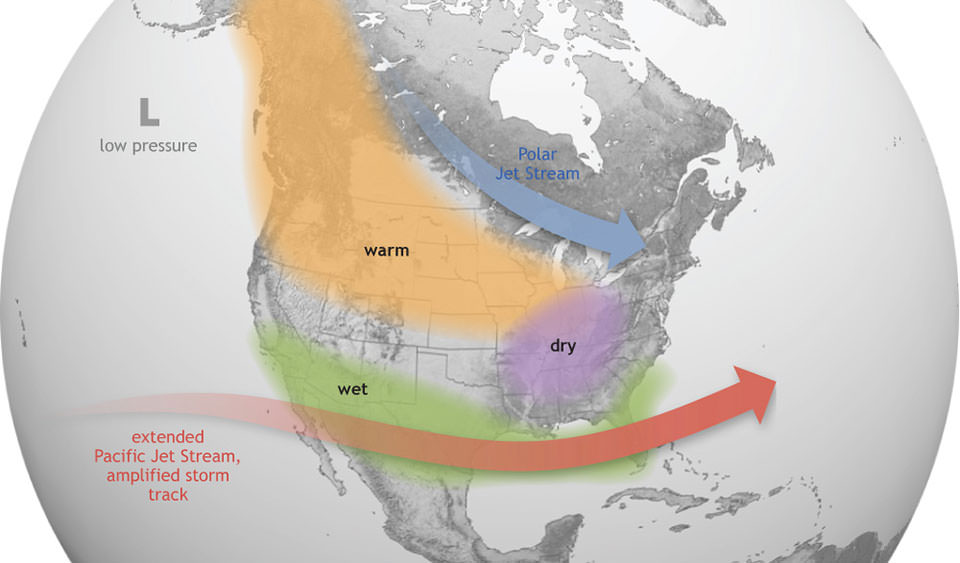
\includegraphics[width=\linewidth,height=0.67\textheight,keepaspectratio]{slide2a.jpg}
\column{0.48\textwidth}

\includegraphics[width=\linewidth,height=0.24\textheight,keepaspectratio]{slide2b.png}
\vspace{0.35cm}
\begin{itemize}\setlength\itemsep{0.75em}
\item ENSO como predictor anticipador de gran escala.
\item ¿Las interacciones de ENSO con zona y elevación afectan SWE?
\end{itemize}
\end{columns}
\end{frame}

\begin{frame}{Dataset}
\begin{center}
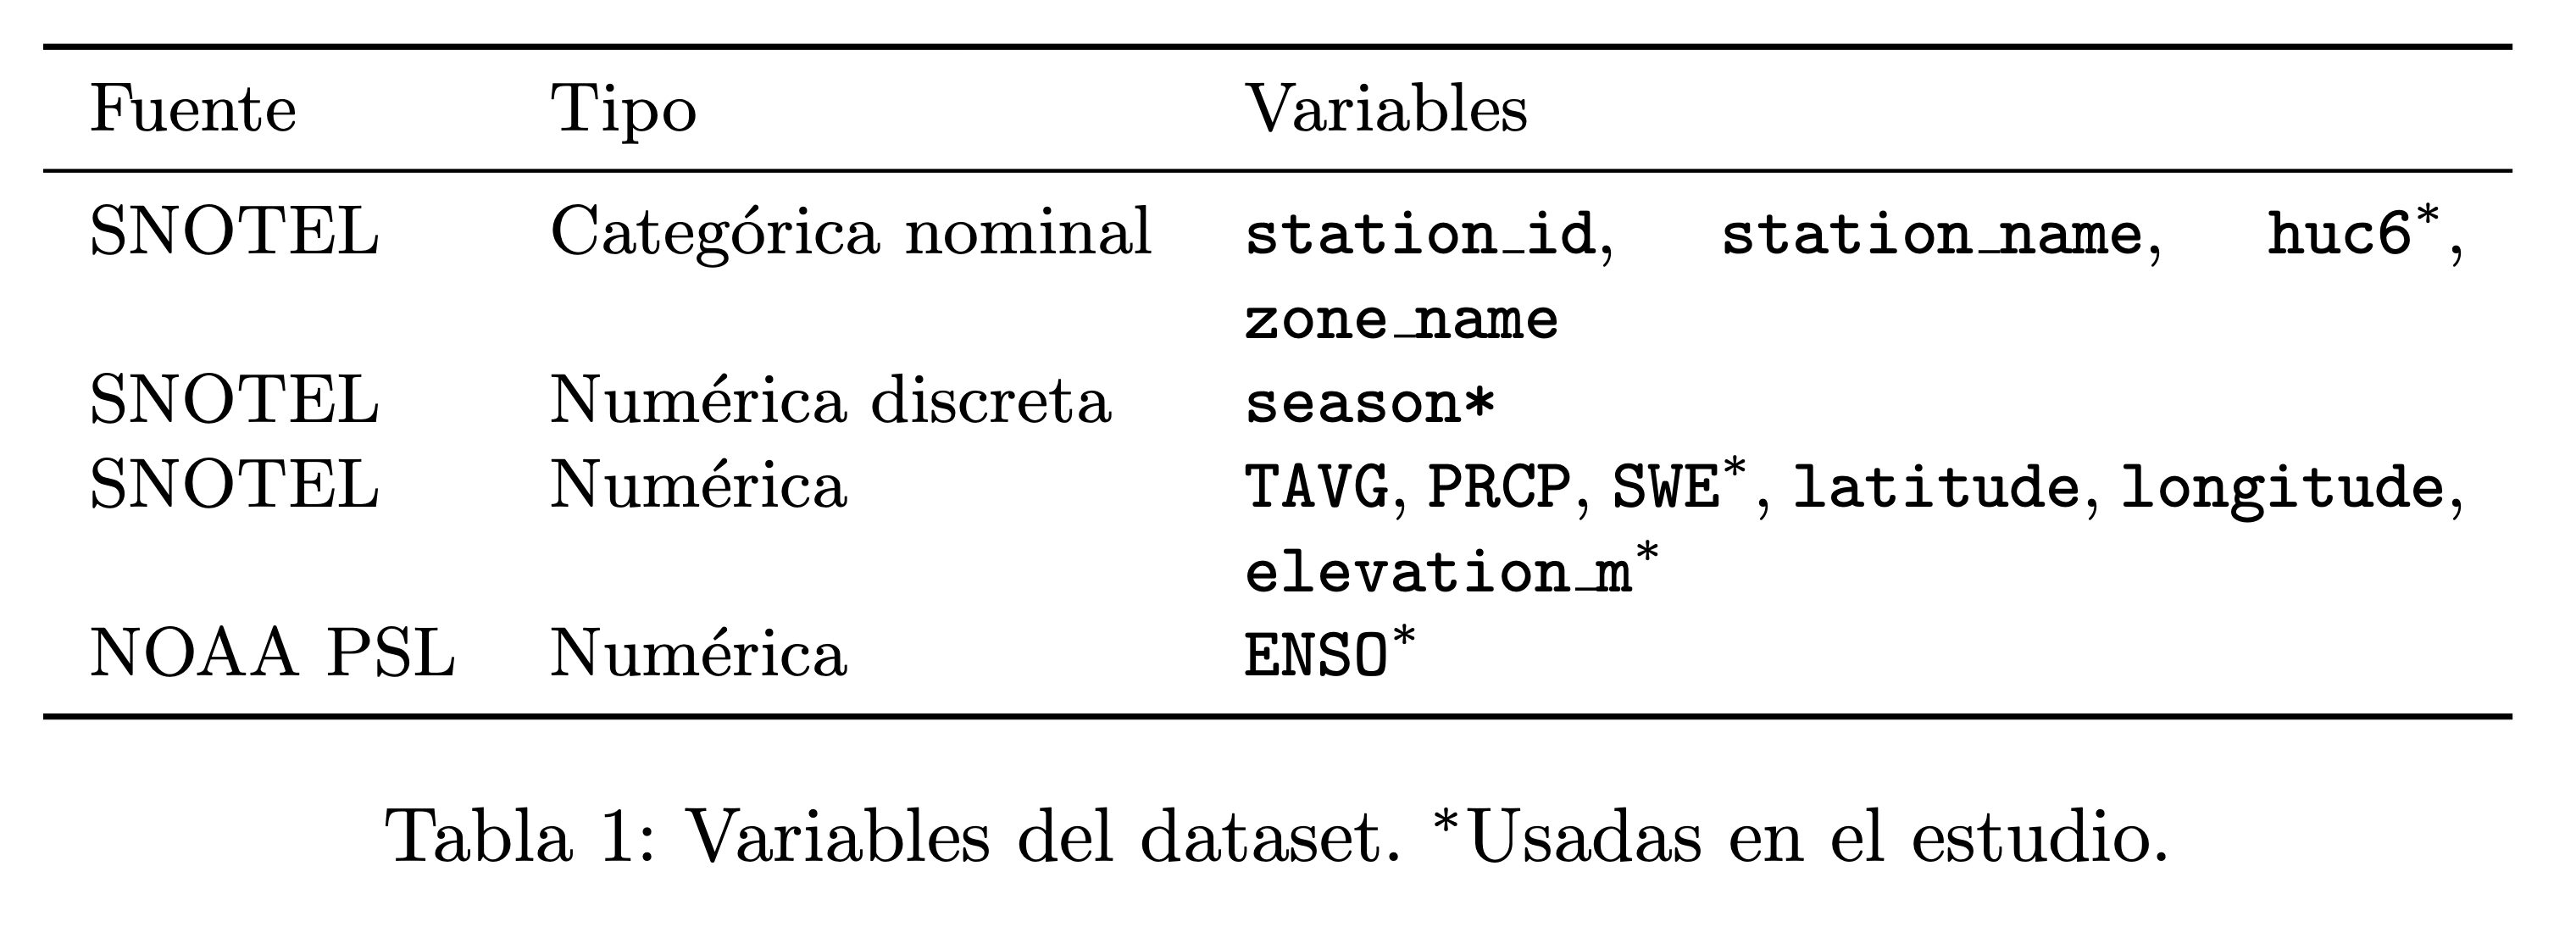
\includegraphics[width=0.78\linewidth,height=0.72\textheight,keepaspectratio]{slide3.png}
\end{center}
\end{frame}

\begin{frame}{Objetivos}
\begin{center}

\includegraphics[width=0.76\linewidth,height=0.25\textheight,keepaspectratio]{slide4.png}
\end{center}
\vspace{0.12cm}
\begin{columns}[T,onlytextwidth]
\column{0.31\textwidth}
\textbf{O1: \textquestiondown Qué puntos existen?}
\begin{itemize}
\item Unidad temporal
\item Agregación
\end{itemize}
\column{0.31\textwidth}
\textbf{O2: \textquestiondown Qué puntos sirven?}
\begin{itemize}
\item Mediciones incompletas
\item Puntos por bloque
\end{itemize}
\column{0.31\textwidth}
\textbf{O3: \textquestiondown Cómo usamos los puntos?}
\begin{itemize}
\item Transformaciones
\item Modelo
\end{itemize}
\end{columns}
\end{frame}

\begin{frame}[shrink=4]{O1 (1/2)}
\begin{columns}[T,onlytextwidth]
\column{0.58\textwidth}
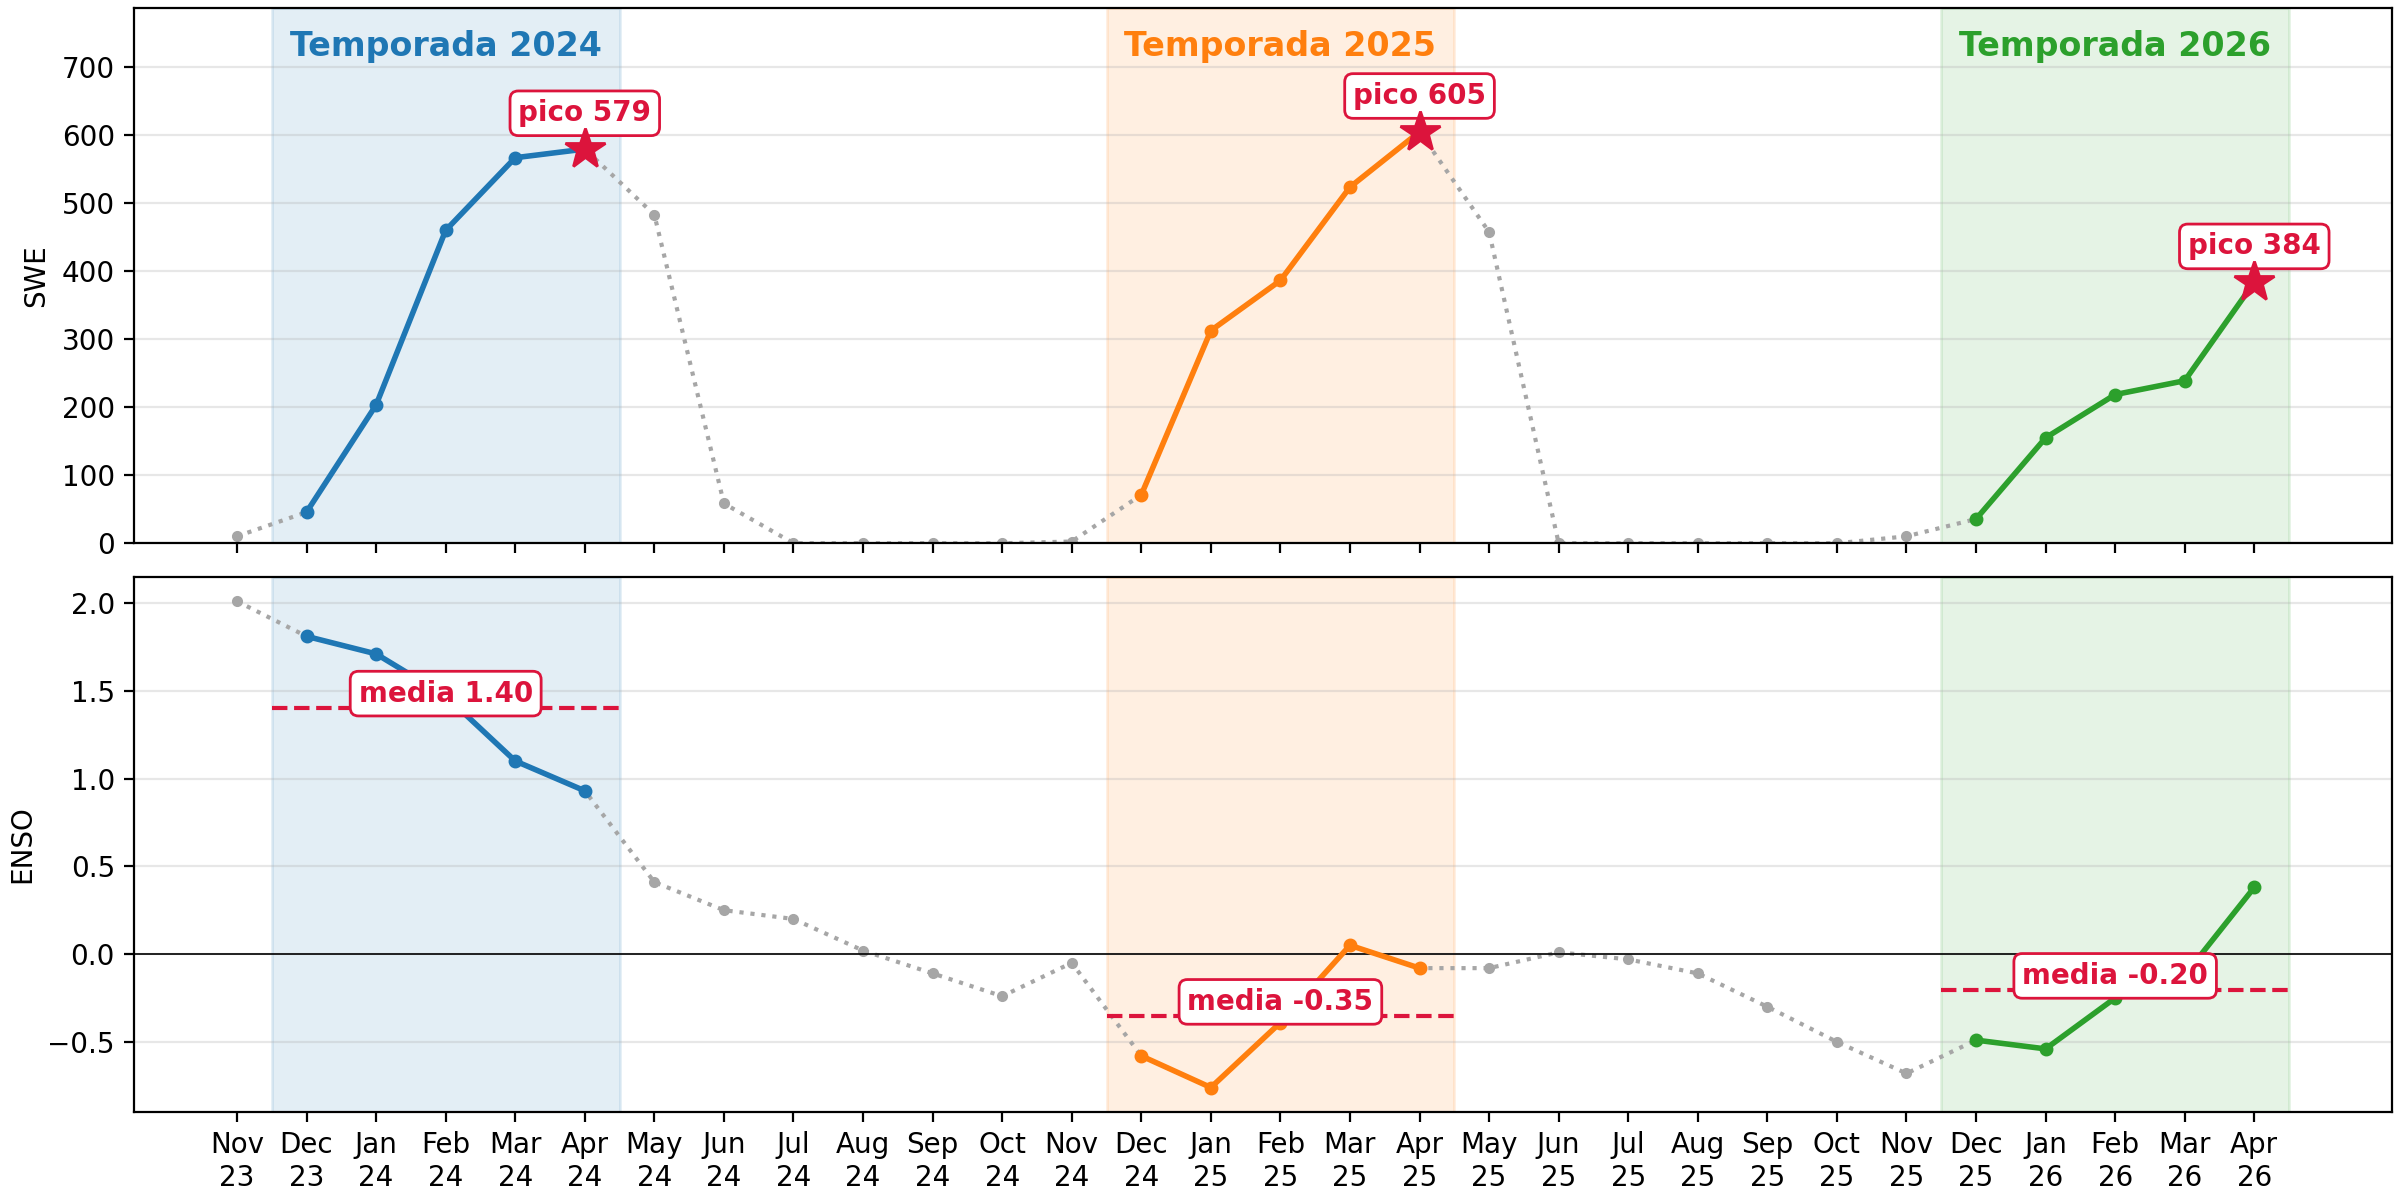
\includegraphics[width=\linewidth,height=0.66\textheight,keepaspectratio]{slide5a.png}
\column{0.38\textwidth}
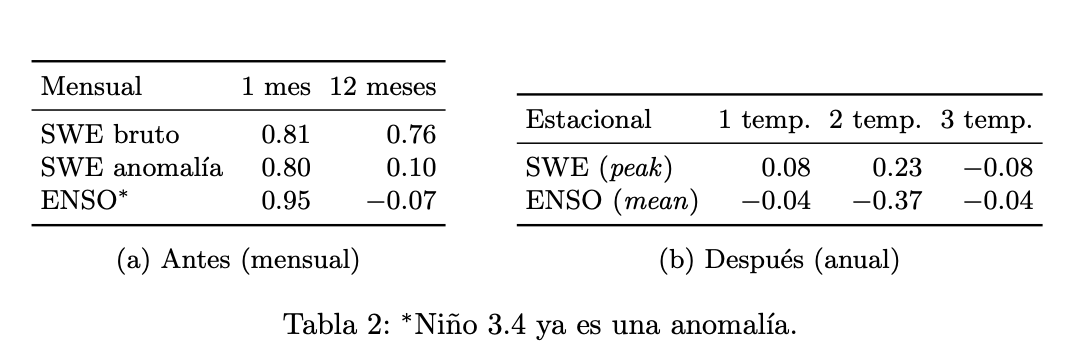
\includegraphics[width=\linewidth,height=0.26\textheight,keepaspectratio]{slide5b.png}
\vspace{0.35cm}
\begin{itemize}\setlength\itemsep{0.55em}
\item Fuerte autocorrelación mensual.
\item Condensación estacional.
\end{itemize}
\end{columns}
\end{frame}

\begin{frame}[shrink=5]{O1 (2/2)}
\begin{center}
\begin{tabular}{>{\bfseries}l l p{0.43\linewidth}}
\toprule
Variable & Agregación & Criterio\\
\midrule
SWE (mm) & Máximo & Pico estacional acumulado\\
TAVG ($^\circ$C) & Media & Persistencia térmica mensual\\
PRCP (mm) & Suma & Volumen estacional acumulado\\
ENSO ($^\circ$C) & Media & Estado climático estacional\\
Zona & Constante & Unidad nominal HUC6\\
Elevación (m) & Constante & Gradiente físico de estación\\
\bottomrule
\end{tabular}
\end{center}
\end{frame}

\begin{frame}[shrink=5]{O2 (1/2)}
\begin{columns}[T,onlytextwidth]
\column{0.48\textwidth}
\textbf{Mediciones incompletas}
\begin{itemize}\setlength\itemsep{0.75em}
\item Si falta un mes, el máximo SWE puede subestimar el pico real.
\item Eliminar solo sesga si las faltas dependen de ENSO.
\item ENSO y fracción descartada: $\rho=0.1105$, p-val.\,$=0.4646$.
\end{itemize}
\column{0.48\textwidth}
\vspace{0.2cm}
\textbf{Imputación}
\begin{itemize}\setlength\itemsep{0.75em}
\item Desde otras estaciones: compartiría información espacial.
\item Desde otras temporadas: modificaría la señal estacional.
\item Sin imputación: evita pseudo-observaciones; se conservan cinco meses (3.30\% descartado).
\end{itemize}
\end{columns}
\end{frame}

\begin{frame}[shrink=5]{O2 (2/2)}
\begin{columns}[T,onlytextwidth]
\column{0.48\textwidth}
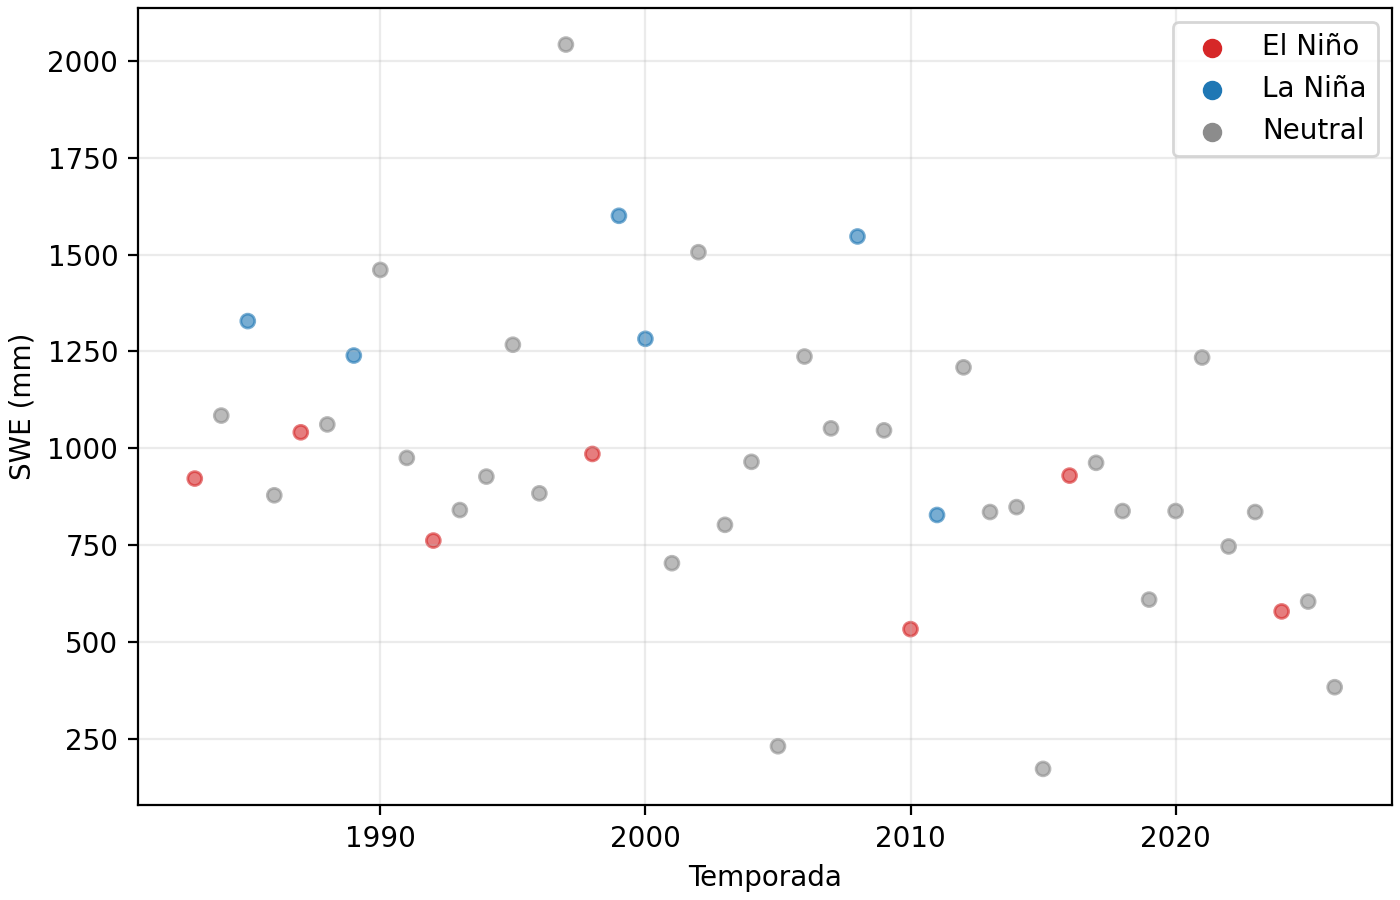
\includegraphics[width=\linewidth,height=0.40\textheight,keepaspectratio]{slide8a.png}
\column{0.48\textwidth}
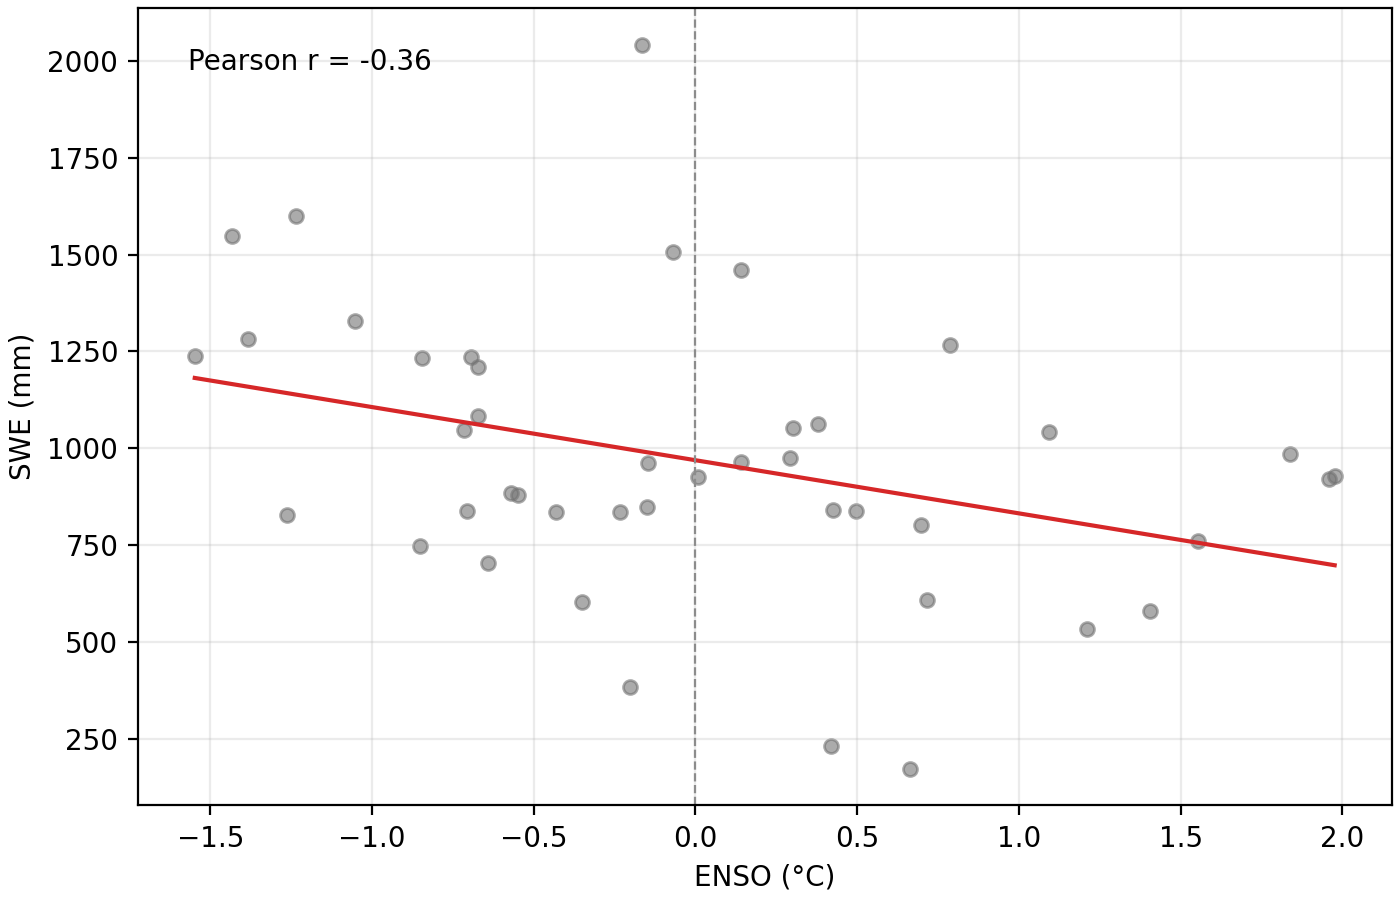
\includegraphics[width=\linewidth,height=0.40\textheight,keepaspectratio]{slide8b.png}
\end{columns}
\vspace{0.25cm}
\begin{columns}[T,onlytextwidth]
\column{0.48\textwidth}
\begin{itemize}\setlength\itemsep{0.35em}
\item La Niña suele superar a El Niño.
\item Hay variabilidad y valores atípicos.
\item Existe tendencia descendente.
\end{itemize}
\column{0.48\textwidth}
\begin{itemize}\setlength\itemsep{0.35em}
\item Suficientes puntos temporales: $\geq30$ temporadas.
\item Suficiente dispersión: se conserva variabilidad ENSO.
\item Eliminación aplicada: 11.085 $\rightarrow$ 10.021 filas.
\end{itemize}
\end{columns}
\end{frame}

\begin{frame}{O3 (1/2)}
\begin{center}
\begin{tabular}{>{\bfseries}l l p{0.46\linewidth}}
\toprule
Original & Transformada & Razón\\
\midrule
SWE & $\log(1+\mathrm{SWE})$ & Conserva ceros; asimetría $1.2365\rightarrow-1.7669$.\\
ENSO & Continua en $^\circ$C & Conserva magnitud; asimetría $0.4533$.\\
Elevación & Baja / media / alta & Umbrales 1500 y 2100 m.\\
Zona & Nominal HUC6 & No impone orden; $\chi^2=160.7883$, p-val.\,$=4.319\times10^{-19}$.\\
\bottomrule
\end{tabular}
\end{center}
\end{frame}

\begin{frame}{O3 (2/2)}
\vspace{1.0cm}
\begin{center}
\textbf{El ANOVA de tres vías no puede validarse en este informe.}\\[0.30cm]
\thintext{Shapiro--Wilk: p-val.\,$=8.17\times10^{-60}$; Breusch--Pagan: p-val.\,$=8.994\times10^{-151}$; 46 valores ENSO comunes.}
\end{center}
\end{frame}

\begin{frame}{Conclusión (1/2)}
\begin{columns}[c,onlytextwidth]
\column{0.60\textwidth}
\begin{center}
\begin{tabular}{c|cccc}
\textbf{Bloque} & SWE & ENSO & Elevación & Zona\\
\hline
{\color{blue}\textbf{Estaciones-temporadas 1}} &
{\color{blue}\rule{0.65cm}{0.65pt}} &
{\color{blue}\rule{0.65cm}{0.65pt}} &
{\color{blue}\rule{0.65cm}{0.65pt}} &
{\color{blue}\rule{0.65cm}{0.65pt}}\\
 & \multicolumn{4}{c}{\color{blue}\rule{4.8cm}{0.65pt}}\\
 & \multicolumn{4}{c}{\color{blue}\rule{4.8cm}{0.65pt}}\\
{\color{orange}\textbf{Estaciones-temporadas 2}} &
{\color{orange}\rule{0.65cm}{0.65pt}} &
{\color{orange}\rule{0.65cm}{0.65pt}} &
{\color{orange}\rule{0.65cm}{0.65pt}} &
{\color{orange}\rule{0.65cm}{0.65pt}}\\
 & \multicolumn{4}{c}{\color{orange}\rule{4.8cm}{0.65pt}}\\
 & \multicolumn{4}{c}{\color{orange}\rule{4.8cm}{0.65pt}}\\
{\color{green}\textbf{Estaciones-temporadas 3}} &
{\color{green}\rule{0.65cm}{0.65pt}} &
{\color{green}\rule{0.65cm}{0.65pt}} &
{\color{green}\rule{0.65cm}{0.65pt}} &
{\color{green}\rule{0.65cm}{0.65pt}}\\
 & \multicolumn{4}{c}{\color{green}\rule{4.8cm}{0.65pt}}\\
 & \multicolumn{4}{c}{\color{green}\rule{4.8cm}{0.65pt}}\\
\end{tabular}
\end{center}
\column{0.36\textwidth}
\begin{itemize}\setlength\itemsep{0.75em}
\item Tamaño efectivo: 46 temporadas ENSO compartidas.
\item Alternativa: remuestreo por bloque estacional.
\end{itemize}
\end{columns}
\end{frame}

\begin{frame}{Conclusión (2/2)}
\begin{center}
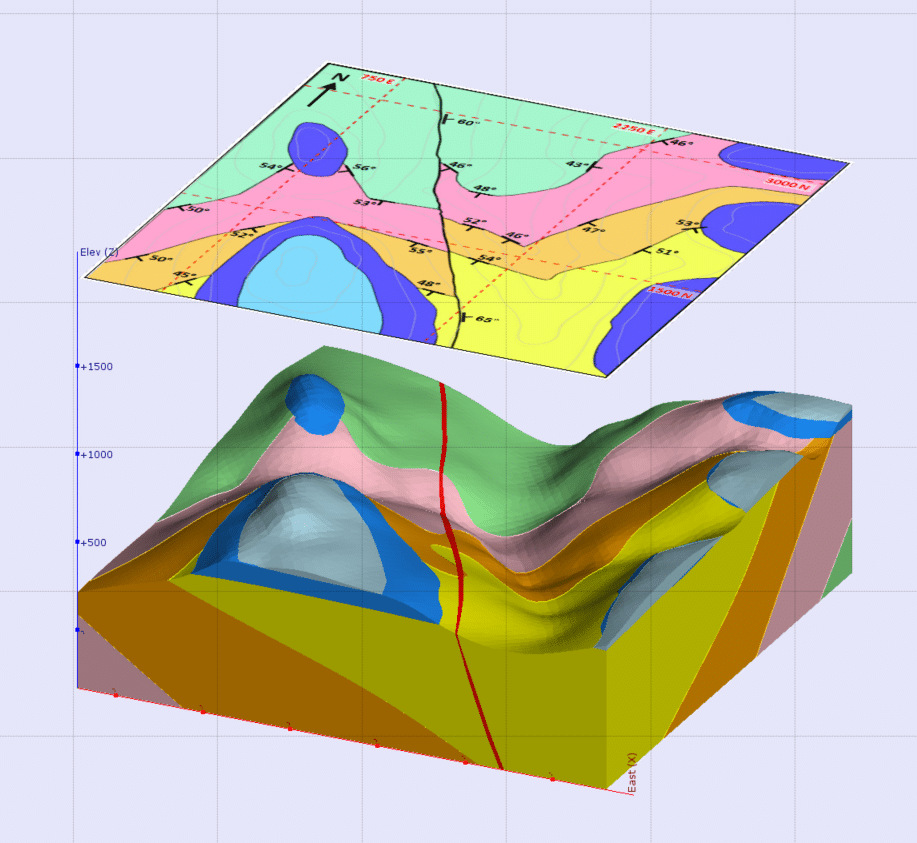
\includegraphics[width=0.72\linewidth,height=0.62\textheight,keepaspectratio]{slide12.png}\\[0.35cm]
\textbf{Análisis geoespacial y temporal}
\end{center}
\end{frame}

\begin{frame}{Referencias}
\begin{itemize}\setlength\itemsep{0.75em}
\item \textbf{NOAA.} Understanding Climate: Oceanic Niño Index.
\item \textbf{NOAA Physical Sciences Laboratory.} Monthly Niño 3.4 anomaly index.
\item \textbf{USDA NRCS.} Air and Water Database (AWDB) REST API.
\item \textbf{Mote, P., Hamlet, A. y Salathé, E.} (2008). Has spring snowpack declined in the Washington Cascades?
\item \textbf{USDA NRCS.} Interactive Map: snow water equivalent.
\end{itemize}
\end{frame}

\end{document}
